\documentclass[11pt]{article}
\usepackage[a4paper,margin=28mm]{geometry}
\usepackage{amsmath,amssymb,amsthm,mathtools,microtype,mathrsfs,tikz}
\usetikzlibrary{arrows.meta,positioning,calc}
\usepackage[colorlinks=true,linkcolor=blue!55!black,citecolor=blue!55!black,urlcolor=blue!55!black]{hyperref}
\numberwithin{equation}{section}
\newtheorem{theorem}{Theorem}[section]
\newtheorem{lemma}[theorem]{Lemma}
\newtheorem{proposition}[theorem]{Proposition}
\newtheorem{corollary}[theorem]{Corollary}
\theoremstyle{definition}\newtheorem{definition}[theorem]{Definition}
\newcommand{\ii}{\mathrm i}
\newcommand{\Z}{\mathcal Z}
\newcommand{\Kern}{\mathcal K}
\title{Meridian expansions and classical symbols of quantum recurrences}
\author{}\date{}
\begin{document}
\maketitle
\begin{abstract}
For fixed strict Conway diagrams with independently long powers, and
for circle trees satisfying a summed or directed degree--twist
criterion, we prove meridian expansions to every inverse-level
order. They hold on fixed translated microscopic charts and retain
the full normal coordinates at repeated spectral roots. At order
$N^{-r}$ the logarithmic coefficient has degree at most $r+1$ in
the microscopic parameter. Its highest degree is the stationary
value of an explicit analytic deformation of the original source.
We then prove that every specified fixed recurrence annihilating
the whole reduced invariant at all sufficiently large levels has
this analytic characteristic germ in its first nonzero classical
symbol. The reduced-to-full gauge retains both its meridian divisor
and its sign. A separate marked geometric identification determines
when the germ is the preferred meridian--longitude branch.
\end{abstract}

\section{Fixed diagrams, normalization and conclusions}\label{me:intro}
Throughout, a diagram is one fixed literal ordered tangle expression,
with its physical turns, original crossing circles, endpoint orders,
cut and zero-framing convention. Its closure is one knot and no
component is closed inside a proper tangle. All signed integer
crossing powers $n_v$ are fixed before $N$ tends to infinity. We use
one of the following already proved source classes:
\begin{enumerate}
\item a strict Conway expression with at least two original circle
vertices and all $|n_v|$ above the single diagram-dependent threshold
of \cite[Theorem 1.2]{MovingSources};
\item an all-circle tree with at least one edge, degrees $d_v$ and
$\sum_v d_v/(d_v^2+n_v^2)\le2^{-25}$, as in
\cite[Theorems 1.1--1.2]{CircleTree};
\item an all-circle tree with a root and numbers $c_v$ satisfying
\cite[equations (7.3), (7.8), (7.9), Theorem 1.3]{CircleTree}.
\end{enumerate}
The last is a finite criterion, not a condition on an unknown
invariant. It includes, by \cite[Corollary 1.4]{CircleTree}, the
separate alternative $d_v\ge2^{28}$ or $|n_v|\ge2^{27}$ at every
vertex, and the local condition
$\max_v d_v/(d_v^2+n_v^2)\le2^{-120}$. In these all-circle cases
large degree can permit $n_v=0$. No long-power assumption is added
to them here. The explicit directed inequalities are recalled in
Section~\ref{me:directed}; no summed hypothesis is substituted for
that criterion.

Let $F_N(M)$ be the actual zero-framed reduced state of
\cite{Meridian}, with $q_N=e^{\pi\ii/N}$ and marked meridian
$M=q_N^s$. In its highest-weight coordinate the pointing is
$M=-q_Nx$; the source flag has eigenvalue $M^{-1}$. Put
\begin{equation}\label{me:normalization}
 K_N=F_N(1),\qquad H_N(s)=\frac{\sin\pi s}{N\sin(\pi s/N)},
 \qquad \Z_N(s)=\frac{F_N(q_N^s)}{K_NH_N(s)}.
\end{equation}
The value of $H_N$ at zero is one. The imported source theorems
prove $K_N\ne0$ for all sufficiently large levels, in both parities.
For $N\ge3$ it is the reduced Kashaev value with the fixed complete
normalization. The one factor $H_N$ is the actual reduced/full
conversion, not an adjustable regularization.

The local action needs its full normalization. Let $X$ collect
all original physical wire coordinates $x_e$, all hidden unturned
product coordinates where present, and the original circle angles
$\tau_v$. Define
\begin{align}
 J(x)&=\int_0^x\log(2\sin\pi u)\,du,\notag\\
 b(x,\tau)&=\int_0^x\log(2\cos2\pi u+2\cos\tau)\,du-2J(x),\notag\\
 m(x,y,z)&=J(x+y)+J(z)-J(x)-J(y)
                 -J(z-x)-J(z-y)-J(x+y-z).\label{me:local-actions}
\end{align}
The logarithms continue the original positive complete branch.
For strict Conway sources retain the complete bare gates and set
\begin{equation}\label{me:base-action}
 \Phi(X)=\sum_{\text{bare gates}}m(x,y,z)
  +\sum_{v\text{ circle}}\sum_{e\ni v}b(x_e,\tau_v)
  +\frac{\ii}{4\pi}\sum_vn_v\tau_v^2-\ii\sum_v\tau_v.
\end{equation}
For all-circle trees the first sum is absent. The last term is the
original first Fourier charge and is part of the mark. Write $X_0$
for its selected filled critical point. The source theorems prove
its nondegeneracy; in the directed case the joint statement follows
also from the conditional Hessians in Section~\ref{me:directed}.
Let $\mathcal E_T$ denote only the original physical turn edges,
not the hidden unturned resolution wires. Set
\begin{align}
 \Kern(x,t)&=2J(x)-J(x+t)-J(x-t),\notag\\
 a(D)&=-w(D)-\sum_v n_v,\notag\\
 \Phi_t(X)&=\Phi(X)+\sum_{e\in\mathcal E_T}\Kern(x_e,t)
                          +\frac{\pi\ii a(D)}2t^2,\label{me:deformed-action}\\
 S(t)&=\Phi_t(X_*(t)),\qquad X_*(0)=X_0.\notag
\end{align}
The analytic implicit function theorem defines this stationary
branch for small $t$. It is an auxiliary local family, not an
assertion about the physical invariant with $s=Nt$.

\begin{theorem}[All orders on translated microscopic charts]
\label{me:all-orders}
For each source above, every $L\ge1$, every compact disk
$|s|\le R<1$, and every fixed compact $K$ in the open upper
half-plane,
\begin{equation}\label{me:expansion}
 \log\Z_N(s)=\sum_{r=1}^L N^{-r}p_r(s)+O(N^{-L-1}),
 \qquad \deg p_r\le r+1.
\end{equation}
The logarithm is the branch tending uniformly to zero. The estimate
holds with every prescribed finite number of derivatives on smaller
compacts. The coefficients are the same on all these charts. They
may be separated by level parity if a lower amplitude requires it;
their highest-degree coefficients agree. More precisely,
\begin{equation}\label{me:diagonal}
 [s^{r+1}]p_r(s)=[t^{r+1}](S(t)-S(0)).
\end{equation}
All coefficient polynomials are even and vanish at zero. In particular
\begin{equation}\label{me:first-coefficient}
 p_1(s)=\frac12S''(0)s^2,\qquad
 S''(0)=\pi\ii a(D)-2\pi\sum_{e\in\mathcal E_T}\cot(\pi x_e(X_0)).
\end{equation}
The constants can depend on the fixed diagram, powers, certificate,
compact, derivative order and expansion order.
\end{theorem}

A recurrence here means a specified finite operator
\begin{equation}\label{me:operator}
 P(q,M,T)=\sum_{j=0}^{r_P}a_j(q,M)T^j,\qquad TM=qMT,
 \qquad a_j\in\mathbb C(q,M),
\end{equation}
which annihilates the whole reduced function $F_N(M)$ for every
sufficiently large integer level. Neither interpolation from finitely
many levels nor an equation for the values $F_N(1)$ is this hypothesis.
Negative shifts can first be removed by multiplication by a power
of $T$. Clear its fixed rational denominators and divide by the
largest common power of $q-1$. Its nonzero specialization is
$P_0(M,L)$. No existence claim for a recurrence is needed for the
following implication.

\begin{theorem}[A classical germ forced by the actual recurrence]
\label{me:symbol}
For every operator \eqref{me:operator} with the stated all-level
property, define
\[
 \mathcal S(u)=\pi\ii\{S(u/(\pi\ii))-S(0)\},\qquad
 L_{\rm an}(e^u)=-e^{\mathcal S'(u)}.
\]
Then $P_0(e^u,L_{\rm an}(e^u))=0$ as a holomorphic germ. Moreover,
writing $M=e^{\pi\ii t}$ and $E_e(M)=e^{2\pi\ii x_e(X_*(t))}$,
\begin{equation}\label{me:longitude-formula}
 L_{\rm an}(M)=-M^{a(D)}\prod_{e\in\mathcal E_T}
                          \frac{M^2-E_e(M)}{1-M^2E_e(M)}.
\end{equation}
The selected irreducible Laurent-polynomial factor of this germ
therefore divides every such $P_0$. This conclusion does not
identify a full polynomial, multiplicity or recurrence ideal.
\end{theorem}

The analytic assertion is proved without a representation-variety
argument. Section~\ref{me:geometric} states the additional marked
geometric input that identifies $L_{\rm an}$ with the preferred
longitude, rather than identifying two germs from a common tangent.

The broader comparison of quantum recurrences with peripheral curves
is the subject of the AJ conjecture. In its colored-Jones formulation,
the conjecture compares the minimal color-shift recurrence at $q=1$
with the $A$-polynomial, with the coordinate convention and factors
depending only on the meridian treated explicitly
\cite[Section 2.2, Conjecture 2]{AJ}; see also the factor formulation
in \cite[Section 1.1]{DiagrammaticAJ}. Here the hypothesis is an operator
identity for the whole meridian function at every sufficiently large
root-of-unity level. The conclusion selects one analytic germ and,
after the separate geometric argument, its preferred-longitude factor.
It neither supplies that operator nor identifies the minimal
colored-Jones recurrence or the other character components. These
references explain the comparison; their proofs are not inputs below.

\section{Finite source estimates on the shifted charts}\label{me:analytic}
The exact moving finite calculus is imported from
\cite[Proposition 6.1, Theorem 7.1 and Proposition 8.1]{Meridian}:
these are respectively the full crossing polynomial and trace,
the original tree contraction, and its scalar ledger. In its fixed
Newton basis, with $d=N-1$,
\[
 e_k(z)=S_k^{-2}\prod_{j<k}(c_j-z),\quad
 S_k=\prod_{r=1}^k2\sin(\pi r/N),\quad
 c_j=2\cos((2j+1)\pi/N),
\]
the quotient is $P_\sigma=\mathsf T_N+2\cos2\pi\sigma$,
$\mathsf T_N(u+u^{-1})=u^N+u^{-N}$. The metric is
$\phi_\sigma(e_i e_j)=\mathbf1_{i+j=d}$ with
$\phi_\sigma=(-1)^dN^2[z^d]\operatorname{rem}_{P_\sigma}$.
An original physical edge, in lower-index convention, has equal
indices and coefficient $\gamma_{e,N}(s)H_N(s)/W_k(s)$, where
\begin{equation}\label{me:W}
 W_k(s)=\prod_{r=1}^k
       \left(1-\frac{\sin^2(\pi s/N)}{\sin^2(\pi r/N)}\right),
 \qquad\gamma_{e,N}\in\{1,q^{s^2/2},q^{-s^2/2}\}.
\end{equation}
The complete Hermite norm uses all distinct node values and the
first derivative at each double node. The odd node $-2$ is simple.
Polynomial equivalence with interval and Chebyshev norms is
\cite[Lemma 2.1]{Bounds}; quotient products of fixed valence are
first reduced, so the assertion does not identify the full matrix
algebra with a commutative polynomial algebra.

\begin{lemma}[Translated compact sets]\label{me:translated}
For every source class in Section~\ref{me:intro}, the local selected
source, its nonzero leading coefficient, and all fixed exponential
error margins hold on a fixed compact $K\subset\{\Im s>0\}$.
Only bounded or polynomial prefactors and starting levels change.
The same is true on a finite union of translates $K+j$.
\end{lemma}
\begin{proof}
For strict Conway sources this is part of
\cite[Theorems 1.1--1.2]{MovingSources}. We give the finite argument
also needed for the all-circle classes. Euler's sine product gives
\begin{equation}\label{me:subset}
 W_k(s)=\prod_{\substack{1\le r\le k\\a\in\mathbb Z}}
                  \left(1-\frac{s^2}{(r+aN)^2}\right).
\end{equation}
The nonzero integers are distinct. On $K\cup(-K)$ the finitely
many small factors are bounded above and away from zero, and the
logarithms of all remaining factors are bounded by $C_K/m^2$.
Products of the minima with one and maxima with one give bounds
for every subset, uniformly in $N,k$. Thus $W_k$, its inverse,
$H_N$ and its inverse are uniformly bounded. Positivity in the
all-circle estimates is used only for the complete Newton factors;
these bounded multipliers do not change their exponential budgets.

For clarity the exact fixed-power interpolation is
\begin{equation}\label{me:crossing}
 r_{N,\sigma}^{[n]}(z)=
 -\frac1{N(U-U^{-1})}\sum_{j=0}^{N-1}
 \lambda_j^n(t_j-t_j^{-1})\frac{P_\sigma(z)}{z-c_j(\sigma)},
\end{equation}
where $U=e^{2\pi\ii\sigma}$,
$t_j=q^{-2j-1+2\sigma}$, $c_j(\sigma)=t_j+t_j^{-1}$ and
$\lambda_j=(-1)^jq^{j(j+1)-2\sigma j}$.
The full power includes $\kappa_\sigma^n$ with
$\kappa_\sigma=q^{(d+\sigma)^2/2}$. The denominator is bounded
away from zero on the nonreal compact. Nodes are in a Chebyshev
ellipse of angular height $O_K(1/N)$. The divided difference and
its derivative have polynomial bounds there, while the fixed
positive or negative powers of the eigenvalues and carrier have
bounded modulus. This proves the same full-polynomial bounds as
on a disk. Exact Chebyshev folding costs a bounded factor per
fold; the number of folds is fixed by the vertex valence.

At a constant opposite-color vertex keep a separate formal
$\sigma$ and use its whole trace on a parameter circle avoiding
collisions. Its confluent normals are removable by the finite
crossing theorem. The maximum principle for the whole trace
minus its finite approximation brings this formal parameter to
zero, while the edge parameter $s$ stays independent. This is not
an identification of constant and moving orientation types.

The actual trace grid is shifted by $2\pi\sigma/N$. Its exact
pole kernel has vertical-side value
$\ii N e^{-Nv}/(1+e^{-Nv})$ after that translation. Thus the
endpoint action loss survives the $O_K(1/N)$ displacement. A
translated chart $s+j$ may wrap finitely many grid points across
$\pm\pi$; retain those entries and their chirps. Their endpoint
loss persists, but the chirp itself is not periodic. Paired charge
coefficients are
\begin{equation}\label{me:charge}
 (-1)^{d(\ell-1)}U_{\ell-1}(\cos2\pi\sigma),\qquad
 |U_{\ell-1}(\cos2\pi\sigma)|
       \le\ell e^{2\pi|\Im\sigma|(\ell-1)}.
\end{equation}
The added fixed exponential in $\ell$ is absorbed by the original
$e^{-N\ell y}$ tail at every fixed positive contour height $y$.
The first coefficient stays exactly one. Real/strip estimates
in \cite[Sections 2--6]{Summed} and the conditional estimates in
\cite[Sections 3--7]{Directed} use precisely these bounded
multipliers, polynomial finite norms and geometric tails. All
exponential margins therefore persist. This verifies their source
hypotheses on $K$ directly; it is not analytic continuation of
an asymptotic estimate through resonant real parameters.
\end{proof}

\begin{figure}[t]
\centering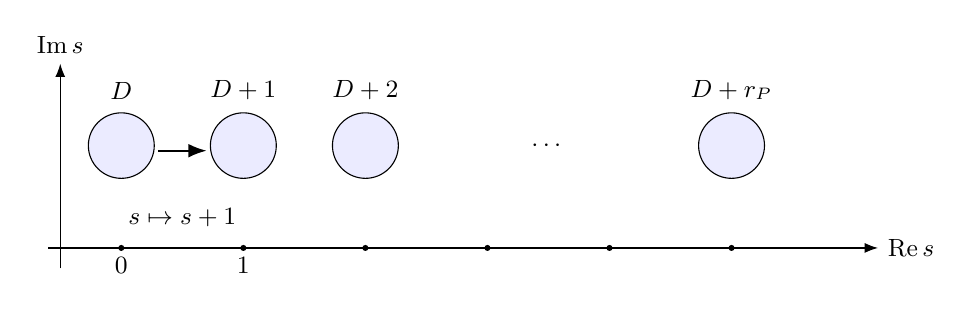
\begin{tikzpicture}[x=1.55cm,y=1.3cm,>=Latex,every node/.style={font=\small}]
\draw[->](-.6,0)--(6.2,0) node[right]{$\operatorname{Re}s$};
\draw[->](-.5,-.2)--(-.5,1.8) node[above]{$\operatorname{Im}s$};
\foreach \j in {0,1,2,3,4,5}{\fill(\j,0)circle(1.1pt);}
\foreach \j/\name in {0/D,1/{D+1},2/{D+2},5/{D+r_P}}{
 \draw[fill=blue!8] (\j,1)ellipse(.27 and .32);
 \node[above]at(\j,1.35){$\name$};
}
\node at(3.5,1){$\cdots$};
\draw[->,thick](.3,.95)--(.7,.95);
\node[below]at(.5,.48){$s\mapsto s+1$};
\node[below]at(0,0){$0$};\node[below]at(1,0){$1$};
\end{tikzpicture}

\caption{A fixed disk $D$ above the real parameter axis and its
translates $D+j$ provide the arguments in an order-$r_P$ recurrence.
The real dots are integer resonances; no contour crosses them.
The physical meridians are $M=q_N^s$, so every fixed disk still
shrinks to $M=1$ as $N$ grows.}
\label{me:chart-figure}
\end{figure}

\section{Canonical local integrals to every order}\label{me:local-orders}
The canonical factorial is
\begin{equation}\label{me:factorial}
 G_N(z)=\left(\frac{2\pi}{N}\right)^z\Gamma(z+1)
 \prod_{a\ge1}\frac{\Gamma(Na+z+1)}
                      {\Gamma(Na-z)(Na)^{2z+1}}.
\end{equation}
We use the complete proof in \cite[Lemma 2.1]{Asymptotics},
including its fixed normalization, sine shift and reflection:
\[
 G_N(k)=S_k,\qquad G_N(z)G_N(N-1-z)=N,
 \qquad G_N(s)G_N(-s)=H_N(s)^{-1}.
\]
On every smaller complex bulk compact it supplies, with all fixed
derivatives and every requested finite order,
\begin{equation}\label{me:factorial-expansion}
 \log G_N(Nx)=NJ(x)+\tfrac12\log(2N\sin\pi x)
           +\sum_{j=1}^{L}N^{-j}b_j(x)+O(N^{-L-1}).
\end{equation}
This is an asymptotic expansion, with no convergence assertion.
The summable Gamma remainders in that lemma justify the infinite
product before differentiation.

The exact local circle factor and the physical edge insertion are
\begin{align}
 \mathcal E_N(x,\tau)&=
 \frac{G_N(d/2+u)G_N(d/2-u)}
 {G_N(d/2-Nx+u)G_N(d/2-Nx-u)G_N(Nx)^2},
 \quad u=\frac{N\tau}{2\pi},\label{me:E}\\
 \mathcal I_N(x,s)&=\frac{G_N(Nx)^2}{G_N(Nx-s)G_N(Nx+s)}.
                                                        \label{me:I}
\end{align}
The sine shift proves their equality with
$e_k(-2\cos\tau)$ and $H_N/W_k$ at $x=k/N$.
In particular the reflection factor in \eqref{me:factorial} puts
$H_N$ in the numerator of the edge weight. Hidden complete gates
are ratios of the same factorials. Every argument, including
$d/2=N/2-1/2$ and every $d-k$ offset, remains exact.

\begin{lemma}[Uniform local expansion]\label{me:local-expansion}
On the selected primitive wire contours and the selected local
angular contours, the canonical integrals have expansions to every
relative inverse-level order. Their coefficients and remainders
are holomorphic on the stated smaller parameter compacts. This
applies to a conditional edge integral with its parent angle still
free, and to a joint strict Conway or summed-circle integral.
\end{lemma}
\begin{proof}
All factorial arguments lie in fixed bulk complex tubes on these
contours. For strict sources this is proved in
\cite[Section 6]{MovingSources}; hidden unturned indices need not
be below half. The exceptional half physical edge is bulk and
causes no pole. For all-circle sources the edge saddle is in the
fixed tube about $1/5<x<3/10$, as proved in
\cite[Section 3]{Summed} and \cite[Section 3]{Directed}.
Substitute \eqref{me:factorial-expansion} into the exact ratios.
Powers of $N$, integer offsets and square-root marks give the
original leading amplitude and complete inverse-power expansions.

The finite lattice is handled before asymptotic integration.
Enclose each primitive coordinate interval by half-grid rectangles
and use $\pi N\cot(\pi Nz)$. On horizontal sides the difference
from its constant value is $O(e^{-2\pi Nh})$; on vertical sides
it is bounded. Choose the height $h$ before the parameter tube,
with the phase gain $C h^2$ less than both a fixed fraction of the
boundary loss and $\pi h$. Thus nonconstant modes and boundary
currents have a fixed exponential loss. The constant terms give
exactly $N^K$ times the local integral, up to those errors. The
primitive lattice and all offsets are the ones in the imported
finite source, so no sublattice multiplicity is introduced.

Translate the local contour to its selected critical point. Its
real quadratic part is uniformly negative on compact parameter
sets; its inverse Hessian and leading amplitude are bounded and
nonzero there. To obtain relative order $L$, Taylor expand phase
and amplitude to a sufficiently high finite order, set
$X-X_*=N^{-1/2}Y$, and split at $|X-X_*|=N^{-\epsilon}$,
with $0<\epsilon<1/6$ chosen first. Outside this shrinking region
the quadratic bound is $e^{-cN^{1-2\epsilon}}$. Inside it expand
the exponential of the cubic and higher terms with its integral
remainder. Taking enough Taylor terms makes that remainder at most
$N^{-L-1}$ times an integrable polynomial times
$e^{-c|Y|^2/2}$. The finitely many Gaussian moments give integer
relative powers: odd total moments vanish. Fixed derivatives are
obtained by starting with more terms and using a smaller tube.

The absolute Gaussian integral is bounded by a constant times the
modulus of its nonzero leading complex integral. Thus a uniform
holomorphic relative remainder stays of the same order after
integration. The bound may depend on fixed degrees and powers,
which is permitted. This proves the claim directly, rather than
promoting a first-order estimate to all orders without a remainder
argument. Conditional angular and edge integrations use the same
proof with the unevaluated parent coordinate as parameter.
\end{proof}

For the strict Conway and summed-circle classes the fixed global
source and charge gaps are already below the same joint first
charge. Lemmas~\ref{me:translated}--\ref{me:local-expansion}
therefore give their entire source to every relative order. The
source error is kept additive until that comparison; it is never
compared with a product of separately damped local contributions.
The directed case requires one additional normalized induction,
which we now give.

\section{All orders in the directed subtree contraction}\label{me:directed}
We recall exactly what the directed certificate controls. Put
$a_0=1/(2\pi)$, $k_0=2^{-16}$, $R_0=1/8$, $b_0=2^{-11}$,
$r_0=1/16$, $t_0=2^{-14}$ and $\chi=1-\cos r_0$.
Choose a root and, at every nonroot vertex, $0<c_v<k_0$ and
$\delta_v=\min\{b_0/2,c_v\chi/[4(1+c_v)]\}$. Let $q_v$ be
one at a nonroot vertex and zero at the root. With children
$\operatorname{Ch}(v)$ define
\begin{align}
 a_v&=\frac{d_v}{2\pi},& b_v&=\frac{n_v}{2\pi},&D_v&=a_v-\ii b_v,
       \notag\\
 A_v&=\frac2{\pi^2}\left(q_vk_0+\frac12\sum_{w\in\operatorname{Ch}(v)}c_w\right),&
 B_v&=16q_v+|\operatorname{Ch}(v)|,&
 C_v&=B_v+\frac{b_v^2}{4A_v}.\label{me:directed-data}
\end{align}
All $A_v,B_v$ are positive because the tree has an edge. Put
$\delta_v^{\rm in}=\min(\{b_0\}\cup\{\delta_w:w\in\operatorname{Ch}(v)\})$,
\begin{align}
 y_v&=\min\left\{\frac{\delta_v^{\rm in}}2,
 \frac{t_0|D_v|}{4C_v},
 \frac{A_v\pi^2}{8(\pi|b_v|+t_0|D_v|)},
 \sqrt{\frac{A_v\pi^2}{8B_v}}\right\},\notag\\
 \beta_v&=\frac{210}{361}\frac{a_v}{|D_v|^2},\qquad
 \eta_v=\min\left\{\tfrac12t_0|D_v|y_v,
 \tfrac12 A_v\pi^2,A_vr_0^2,\tfrac18a_vr_0^2\right\}.
 \label{me:directed-losses}
\end{align}
The criterion is $t_0|D_v|\ge2$ and $\beta_v<\eta_v/2$ at every
vertex, and $\beta_v<(k_0-c_v)\chi$ at each nonroot vertex.
These are the same finite inequalities as in \cite{CircleTree}.

The full edge polynomial is
\begin{equation}\label{me:full-kernel}
 \mathscr K_N(t,u;s)=\sum_{k=0}^{N-1}
       e_k(-2\cos t)e_k(-2\cos u)\frac{H_N(s)}{W_k(s)}.
\end{equation}
Its trigonometric degree in either angle is at most $N-1$;
there is no high-index truncation in this definition. Let
$M_{v,N}(u;s)$ denote the exact polynomial sent by a subtree to
its parent angle $u$. It is the actual trace of the parent kernel
times the exact child messages, with the original typed scalar.
At the root the parent kernel is absent. This is an evaluation
order for a fixed contraction, not a new diagram.

The written induction in \cite[Sections 7.3--7.5]{CircleTree} proves,
on the parent rectangle $|\Re u|\le R_0$, $|\Im u|\le b_0$,
a nonzero conditional first-charge saddle. Its local real second
derivative is at most $-(19/20)a_v$ and its complex Hessian modulus
is at least $(19/20)|D_v|$. All tail, endpoint, truncation and
connector errors are below that first charge by a positive margin
at least $\eta_v-\beta_v$. Each retained charge $\ell\ge2$ has
additional loss
\begin{equation}\label{me:directed-charge-loss}
 \frac{190}{441}\frac{a_v}{|D_v|^2}(\ell^2-1).
\end{equation}
The outgoing real-envelope margin is
$(k_0-c_v)\chi-\beta_v>0$ when an outgoing edge exists. There is
no outgoing requirement at the root. These assertions are the
conditional conclusions of that proof, not consequences inferred
solely from its final scalar asymptotic. The full kernel, all
normal data and the exact child scalars are retained there.
Lemma~\ref{me:translated} verifies these same finite interfaces
on the translated parameter compacts. For one fixed finite tree
all these finitely many positive margins have positive minimum.
The infinite charge tail is one geometric series, not a minimum
of infinitely many unrelated gaps.

\begin{proposition}[Normalized induction to arbitrary order]
\label{me:directed-orders}
Every fixed directed certificate above gives all relative orders
of the actual normalized subtree messages on smaller parent
rectangles and the meridian compacts of Theorem~\ref{me:all-orders}.
Their phase is stationary elimination of \eqref{me:base-action},
with the exact scalar factors restored at the root.
\end{proposition}
\begin{proof}
Strengthen the induction to
\begin{equation}\label{me:message-orders}
 \frac{M_{v,N}(u;s)}{M_{v,N}(0;s)}
 =e^{Nh_v(u)}\frac{\alpha_v(u)}{\alpha_v(0)}
 \left(1+\sum_{j=1}^L N^{-j}a_{v,j}(u,s)
                          +O(N^{-L-1})\right).
\end{equation}
Here $h_v(0)=0$, $\alpha_v$ is nonzero, and the coefficients and
remainders are holomorphic. The exact denominator is nonzero
for all sufficiently large levels by the conditional first-charge
estimate. It is never replaced by an estimate for its modulus.

For a terminal vertex, Lemma~\ref{me:local-expansion} applied to
its full kernel and trace proves \eqref{me:message-orders}; its
complement and currents retain the original positive margins.
Suppose it holds for all children. Their finite product has an
expansion to every chosen relative order, with a nonzero normalized
leading amplitude. On the first-charge local contour use that
expansion and the canonical parent-kernel expansion. The conditional
Hessian and sine factor are nonzero. Absolute Gaussian domination
from Lemma~\ref{me:local-expansion} preserves the relative remainder,
and extra derivatives are obtained by beginning at a higher order.
This proves the first-charge expansion and its exact normalization
at $u=0$.

Outside that contour continue to use the exact child polynomials
and their established real and strip envelopes. Taylor polynomials
for the child expansion are not substituted on a tail. Nonminimal
charges are their local contributions plus additive errors already
below the first charge; a relative expansion at an exponentially
small nonminimal saddle is unnecessary. Inequality
\eqref{me:directed-charge-loss} and the original endpoint and
regeneration margins make these errors smaller than any prescribed
relative inverse power. The outgoing-envelope step again uses the
exact normalized message. It is unaffected by the additional local
Taylor coefficients. This closes the induction on the finite tree.

To identify the joint phase, restore the wire variables in each
parent kernel. Their Hessian blocks are invertible. At each angular
elimination the conditional Hessian is invertible by the displayed
bound. The block determinant identity therefore proves that the
original joint Hessian is invertible, and back-substitution recovers
its selected critical point. No equation for a fixed total action
was guessed from the local critical values. Exact factors
$M_{v,N}(0;s)$ restore every constant subtracted in the normalized
messages. At any finite order, repeated Gaussian integration gives
the same moments as the joint local integral: integrating an
invertible block Gaussian and then its Schur complement is the
usual completion of the square, and differentiation generates all
polynomial moments. The uniform absolute bounds already proved
justify that finite repeated integration. Thus both the phase and
the lower coefficients belong to the original joint source.
\end{proof}

This argument allows constants depending on the fixed tree's size
and depth, as an all-orders theorem for one fixed diagram should.
It neither strengthens the directed criterion nor applies the
summed criterion to a tree which only satisfies local inequalities.

\section{The stationary deformation and the polynomial filtration}
\label{me:filtration}
Set $\delta=1/N$ and introduce an independent small variable $t$.
Equation~\eqref{me:factorial-expansion} gives, to every chosen finite
order,
\begin{equation}\label{me:insertion-log}
 \log\mathcal I_N(x,s)=\delta^{-1}\Kern(x,t)+B_0(x,t)
               +\sum_{j=1}^L\delta^j B_j(x,t)+O(\delta^{L+1}),
 \qquad t=\delta s.
\end{equation}
Each $B_j$ is holomorphic, even in $t$, and zero at $t=0$.
The $\log N$ terms cancel. Explicitly, $B_0$ is half the same
second difference of $\log(2\sin\pi x)$; the further terms are
second differences of the $b_j$. For a literal argument
$x=\ell(X)+\delta c$, expansion of the leading term contributes
$c\Kern_x(\ell,t)$ to $B_0$ and further holomorphic terms to the
lower coefficients. This preserves every $d$ and midpoint offset
without changing the leading phase.

In the local first-charge integral replace the physical insertion
by the same canonical ratio at $s=Nt$ for small independent $t$.
All its arguments remain bulk. This defines an auxiliary analytic
family whose leading phase is exactly
\eqref{me:deformed-action}: the last quadratic term is the exact
scalar $q^{a(D)s^2/2}$. It defines no global asymptotic statement
for a physical parameter growing with $N$. All global estimates
were established for bounded $s$ first. On restricting $t=\delta s$
the auxiliary local family equals the original local integrand.

The joint Hessian of $\Phi$ is invertible, by the source theorem
in the strict and summed cases and by
Proposition~\ref{me:directed-orders} in the directed case. Thus
$X_*(t)$ is analytic and even. Apply the finite-order Gaussian
construction of Lemma~\ref{me:local-expansion} to the auxiliary
local family, uniformly for small $t$. The nonzero leading
amplitude has a fixed local logarithm. It gives holomorphic germs
$C_j(t)$ with
\begin{equation}\label{me:log-family}
 \log\Z_N(s)\sim N\{S(s/N)-S(0)\}
       +\sum_{j\ge0}N^{-j}\{C_j(s/N)-C_j(0)\}.
\end{equation}
The equality means every specified finite truncation with a
uniform asymptotic remainder on the charts already proved.
For the directed proof the iterated local family has precisely
these coefficients: its block stationary elimination and Gaussian
moments were identified in Proposition~\ref{me:directed-orders}.
Exact child constants are restored, not suppressed in
\eqref{me:log-family}. In every class the powers of $N$ and all
$s$-independent scalar factors cancel in the ratio at $s=0$.

Every coefficient in this local family is even in $t$. Uniqueness
of the critical branch preserves that symmetry, as do the exact
edge ratios and the scalar. Hence the $C_j$ and $S$ are even.
Possible lower-coefficient parity dependence can be carried
through this construction separately; its leading phase is the
same. Expand the germs in \eqref{me:log-family}. A term $t^k$ in
$N(S-S(0))$ contributes $N^{1-k}s^k$, while a term $t^k$ in
$N^{-j}(C_j-C_j(0))$ contributes $N^{-j-k}s^k$. At order $N^{-r}$
only the first expression can have degree $r+1$; all the others
have degree at most $r$. This proves the filtration and
\eqref{me:diagonal}. It is a coefficient calculation at every
finite order, not an inference from the first correction.

All discarded terms have fixed exponential losses on each fixed
chart, so they and their fixed derivatives are smaller than every
requested inverse power. The coefficients on translated charts
are the same because they were constructed from the same canonical
local family and scalar. No continuation of an asymptotic estimate
through the real resonances is used. Since $\Z_N\to1$ uniformly
on each chart, the logarithm tending to zero is unique for large
$N$. This proves Theorem~\ref{me:all-orders}.

The first coefficient has no lower-amplitude contribution:
$C_0'(0)=0$ by evenness, and normalization removes the constant.
Moreover $\Phi_{Xt}(X_0,0)=0$, so stationary differentiation gives
\[
 S''(0)=\Phi_{tt}(X_0,0)
       =\pi\ii a(D)-2\sum_eJ''(x_e(X_0))
       =\pi\ii a(D)-2\pi\sum_e\cot\pi x_e(X_0).
\]
This proves \eqref{me:first-coefficient} without a geometric
identification of the resulting complex number.

\section{The exact reduced-to-full gauge}\label{me:gauge}
The full modified dimension in the normalization of
\cite[equation (10.11)]{Finite} is
\begin{equation}\label{me:modified-dimension}
 d_N(M)=\ii^{N+3}\frac{M-M^{-1}}{M^N-M^{-N}},\qquad
 d_N(1)=\frac{\ii^{N+3}}N.
\end{equation}
The value at one is a limit in $M$. It satisfies
$d_N(q_N^s)/d_N(1)=H_N(s)^{-1}$. Thus \eqref{me:normalization}
is the full state divided by its value at one. Write $f(M)=M-M^{-1}$.
Since $q_N^N=-1$, for every integer $j$,
\begin{equation}\label{me:gauge-ratio}
 \frac{d_N(q_N^jM)}{d_N(M)}
          =(-1)^j\frac{f(q_N^jM)}{f(M)},\qquad
 \frac{H_N(s+j)}{H_N(s)}=(-1)^j\frac{f(M)}{f(q_N^jM)}.
\end{equation}
These are exact identities, including the meridian divisor.

Let $P$ be as in \eqref{me:operator}, after clearing its original
rational denominators and removing its common $q-1$ valuation.
Substituting $F_N(q_N^s)=K_NH_N(s)\Z_N(s)$ in its actual equation
shows that $\Z$ satisfies the fixed rational Ore operator
\begin{equation}\label{me:full-operator}
 \widetilde P=\sum_{j=0}^{r_P}a_j(q,M)(-1)^j
                           \frac{f(M)}{f(q^jM)}T^j.
\end{equation}
Multiplication on the left by $\prod_{j=1}^{r_P}f(q^jM)$ clears
these added denominators. The first nonzero classical symbol is
\begin{equation}\label{me:gauged-symbol}
                     f(M)^{r_P}P_0(M,-L).
\end{equation}
It is nonzero as a Laurent polynomial. No meridian factor is
removed by a convention about the reduced invariant.

Choose an open disk $D$ in the upper half-plane and apply
Theorem~\ref{me:all-orders} to slightly enlarged compact disks
covering $D,D+1,\ldots,D+r_P$. The exact cleared equation holds
there for every sufficiently large level, and $\Z$ is nonzero.
Divide by $\Z_N(s)$ and compare successive powers of $N^{-1}$.
The uniqueness of asymptotic coefficients follows by multiplying
by the first putative nonzero power and taking the limit; it holds
along either parity sequence. Every resulting coefficient vanishes
on $D$. Since the coefficient is a polynomial in $s$, obtained
by the finite shifts and the Taylor series of Laurent polynomial
coefficients at $(q,M)=(1,1)$, it vanishes identically.
This step uses expansions at all the shifted arguments of the
actual equation. Complete values or a chart restricted to $|s|<1$
would not justify an operator of arbitrary fixed order.

\section{Recovering the classical characteristic}\label{me:formal}
Put $h=\log q$ and $u=\log M$, so the physical substitution is
$u=hs$ and $h=\pi\ii/N$. The filtration gives a unique regrading
of the formal logarithm as
\begin{equation}\label{me:regrading}
             h^{-1}\mathcal S(u)+\sum_{a\ge0}h^a A_a(u),
 \qquad\mathcal S(u)=\pi\ii\{S(u/(\pi\ii))-S(0)\}.
\end{equation}
Indeed a monomial $h^r s^k$ becomes $h^{r-k}u^k$;
$k\le r+1$ permits just the one negative power $h^{-1}$.
For each exponent of $h$ its coefficient is a formal series in
$u$. Its leading part is fixed by \eqref{me:diagonal}.
Under the $j$th shift, $u$ changes to $u+jh$. The difference of
\eqref{me:regrading} has no negative power of $h$, because
$\mathcal S(u+jh)-\mathcal S(u)$ is divisible by $h$. Its
constant coefficient is $j\mathcal S'(u)$. The lower $A_a$
contribute no constant coefficient. Consequently the formal
shift ratio belongs to $\mathbb C[[h,u]]$ and has constant
$h$-coefficient $e^{j\mathcal S'(u)}$. Its exponential is
well defined because $\mathcal S'(0)=0$.

We give the needed injectivity explicitly. For
$B(h,u)=\sum_{a,b\ge0}B_{a,b}h^au^b$, substitution $u=hs$ gives
\begin{equation}\label{me:coefficient-recovery}
 [h^ns^b]B(h,hs)=
 \begin{cases}B_{n-b,b},&b\le n,\\0,&b>n.\end{cases}
 \qquad B_{a,b}=[h^{a+b}s^b]B(h,hs).
\end{equation}
At each $n$ there are finitely many terms, so this is a well-defined
ring map into $\mathbb C[s][[h]]$, and the second equality proves
injectivity. Agreement through order $h^L$ recovers exactly the
triangle $a+b\le L$, not all coefficients. For example $h^{L+1}$
is invisible at that finite order. We need, and have proved, every
finite asymptotic order.

The formal operator equation from Section~\ref{me:gauge} therefore
holds before substitution. Take its constant $h$-coefficient and
use \eqref{me:gauged-symbol} to obtain
\[
 f(e^u)^{r_P}P_0(e^u,-e^{\mathcal S'(u)})=0.
\]
The ring of formal series is a domain and $f(e^u)$ is nonzero.
Cancel it in this identity, without altering the operator, to get
\begin{equation}\label{me:symbol-identity}
                  P_0(e^u,-e^{\mathcal S'(u)})=0.
\end{equation}
The germ $S$ is analytic by its local implicit construction, so
this formal equality is also an equality of holomorphic germs.

Stationary differentiation of \eqref{me:deformed-action} gives
its exact rational form. With $M=e^{\pi\ii t}$ and
$E=e^{2\pi\ii x}$,
\begin{equation}\label{me:sine-ratios}
 e^{\Kern_x(x,t)}=\frac{(1-E)^2}{(1-EM^2)(1-E/M^2)},\qquad
 e^{\Kern_t(x,t)}=\frac{M^2-E}{1-M^2E}.
\end{equation}
These follow by substituting $2\sin\pi z$ in
$\Kern_x=2J'(x)-J'(x+t)-J'(x-t)$ and
$\Kern_t=J'(x-t)-J'(x+t)$; their logarithms are zero at $t=0$.
The derivative of the stationary value differentiates only the
explicit parameter. Thus
$\mathcal S'(u)=S'(u/(\pi\ii))$ and
\eqref{me:longitude-formula} follows. All denominators are units
near the selected point since the original filled bulk labels
have $E_e\ne1$; a half label $E_e=-1$ is harmless.
This proves the analytic part of Theorem~\ref{me:symbol}.

For any one specified operator in that theorem, evaluation on
this germ is a homomorphism
$\mathbb C[M^{\pm1},L^{\pm1}]\to\mathbb C\{u\}$ with prime
kernel. The kernel is nonzero by \eqref{me:symbol-identity}.
It contains no nonzero Laurent polynomial in $M$ alone because
$M=e^u$ is nonconstant. Its height is therefore one: a height-two
prime in this two-dimensional Laurent polynomial ring would give
an algebraic constant value of $M$. This ring is a unique
factorization domain, so its height-one prime is generated by
one irreducible Laurent polynomial, up to a monomial unit.
Every $P_0$ in the theorem belongs to it. Over a smaller coefficient
field the contraction of this prime can include conjugate factors;
no claim that an individual complex factor is defined over that
field is needed. The conclusion concerns the selected germ and
its factor, not all components or their multiplicities.

\section{Identifying the preferred longitude}\label{me:geometric}
The preceding theorems construct an analytic characteristic from
an actual source and a specified recurrence. Its geometric
identification uses two separately proved classical statements.
For all-circle trees, \cite[Theorem 1.2 and Corollary 7.1]{Nonparabolic}
construct the full original-group filled germ at its positive
hyperbolic endpoint, with the $M^{-1}$ flag and primitive
logarithms. They give uniqueness after the actual endpoint and
those marks have been identified. For strict sources with bare
junctions, \cite[Theorem 1.3]{Longitudes} identifies the stationary
branch of precisely \eqref{me:deformed-action}, retaining the
original physical edges and all bare junctions. Its proof uses
classical zero-circle insertion and elimination; it includes the
half-label fold and makes no quantum asymptotic assumption.

We spell out the all-circle interface to avoid replacing a group
identification by an equality of second derivatives. Put
$Q_v=e^{\ii\tau_v}$ and $E_e=e^{2\pi\ii x_e}$. Differentiating
\eqref{me:local-actions} and using \eqref{me:sine-ratios}, the
wire stationary equation is exactly
\begin{equation}\label{me:edge-equation}
 (E_e+Q_v)(E_e+Q_v^{-1})(E_e+Q_w)(E_e+Q_w^{-1})
 =(E_e-1)^2(1-E_eM^2)(1-E_e/M^2).
\end{equation}
The local source log satisfies
\begin{equation}\label{me:angle-log}
 -2\pi b_\tau(x,\tau)=
          \log\frac{Q+E}{1+QE}.
\end{equation}
To check its branch as well as its derivative, differentiate both
sides in $x$: both derivatives are
$2\pi\sin\tau/(\cos2\pi x+\cos\tau)$; both sides vanish at
$x=0$. Continue from the same complete chart. The original angle
stationarity therefore gives
\begin{equation}\label{me:primitive}
 \sum_{e\ni v}\log\frac{Q_v+E_e}{1+Q_vE_e}
       -n_v\log Q_v=-2\pi\ii,
 \qquad n_v=\epsilon_v-2p_v.
\end{equation}
These are exactly $U_v+p_vV_v=-2\pi\ii$, with
$U_v=\sum\log((Q_v+E_e)/(1+Q_vE_e))-\epsilon_v\log Q_v$
and $V_v=2\log Q_v$. The linear first-charge term in
\eqref{me:base-action} fixed the right side before exponentiation.

At $t=0$ the selected source point is the positive smooth endpoint
identified by the original summed or directed source theorem;
\cite[Section 8]{Directed} includes its backwards restoration from
conditional saddles. The summed criterion gives
$\sqrt{d_v^2+n_v^2}\ge\sqrt{2^{25}d_v}>630$ at every vertex,
and the directed criterion gives
$\sqrt{d_v^2+n_v^2}=2\pi|D_v|\ge2\pi\,2^{15}>630$.
Thus the marked geometric theorem applies also to high-degree
vertices with zero twist. Its full-group reconstruction uses
\eqref{me:edge-equation} and the original flags, not just traces.
At that endpoint $Q_v^2\ne1$ for each filled disk. It persists on
a neighborhood, so a slope word commuting with its semisimple
longitude and having eigenvalue ratio one is projectively identity.
Consequently the reconstructed branch is a branch of the actual
filled group. The endpoint, flag and primitive logarithmic
conditions now meet the hypotheses of
\cite[Corollary 7.1]{Nonparabolic}, which identifies the branch.

For the geometric conclusion in the strict class, enlarge its
fixed power threshold to the maximum of the analytic threshold in
\cite[Theorem 1.2]{MovingSources} and the classical positive-filling
and longitude threshold in \cite[Theorem 1.3]{Longitudes}. Both
are constants of the same fixed original diagram, so this preserves
independent signed powers and imposes no ratio condition. The
analytic theorems above themselves require only their analytic
source threshold. No inequality between the two thresholds is
being assumed.

For a strict source beyond this common threshold the classical action in
\cite[Theorem 1.3]{Longitudes} is the sum of the same $m$ and $b$
functions, with their absolute primitives, the same chirp and the
same first-charge term. Hidden unturned wires can be retained
before its stationary elimination. Its original physical-edge
set is $\mathcal E_T$. The nondegenerate source branch proved
here therefore equals that classical branch by the local implicit
uniqueness theorem; no individual half-edge elimination is used
at a folded label.

\begin{corollary}[The selected geometric factor]\label{me:geometric-factor}
For every fixed source in Section~\ref{me:intro}, with the strict-class
threshold enlarged to the common threshold just specified, the germ
$L_{\rm an}$ is its preferred-longitude eigenvalue on the $M$
line, equivalently the inverse value on the source $M^{-1}$ line.
It has lift $L_{\rm an}(1)=-1$. Every specified actual all-level
annihilator in Theorem~\ref{me:symbol} contains this selected
geometric factor in its first nonzero classical symbol. If
$\tau_K=\left.\frac{d}{du}\log[-L_{\rm an}(e^u)]\right|_{u=0}$,
then uniformly on the stated charts,
\[
 \frac{F_N(q_N^s)}{K_NH_N(s)}
       =1+\frac{\pi\ii\tau_K s^2}{2N}+O(N^{-2}).
\]
\end{corollary}
\begin{proof}
The branch identification just established permits the marked
longitude formulas \cite[Theorems 1.2--1.3]{Longitudes}. Their
rational product is \eqref{me:longitude-formula}, including its
integer exponent $a(D)$ and negative determinant-one sign. Those
constants are fixed there by peripheral and framing calculations,
not by the quantum tangent. Hence $\tau_K=\mathcal S''(0)
=S''(0)/(\pi\ii)$. Theorem~\ref{me:symbol} proves the factor
statement, and \eqref{me:first-coefficient} gives the expansion.
\end{proof}

\section{Finite reproduction and boundaries}\label{me:checks}
The accompanying \texttt{check.py} checks the finite rational
reduced/full gauge for several operator orders, the rational sine
ratios in \eqref{me:sine-ratios}, and coefficient recovery and
finite-jet truncation for sparse formal polynomials. These are
algebraic checks of displayed identities. They do not establish
analytic remainders, global source gaps, existence of a recurrence,
or a geometric branch by testing levels. Those are the written
proofs and explicitly named companion inputs above.

The expansion is microscopic on each fixed compact in $s$.
The auxiliary $t$ family organizes its local coefficients and
creates an analytic germ, but does not supply a global asymptotic
for fixed $M\ne1$. The recurrence hypothesis is one fixed finite
operator valid for the whole function at all sufficiently large
levels. The conclusion selects one germ and one irreducible factor;
it does not assert equality with a full $A$-polynomial or an
operator ideal. None of these distinctions alters the original
all-level and both-parity source conclusions.

\begin{thebibliography}{10}
\bibitem{Finite}\emph{Finite spectral evaluation and uniform filling bounds}, companion paper,
\href{https://sashakolpakov.github.io/murakamis_dream/papers/filling-bounds.pdf}{repository edition}.
\bibitem{Meridian}\emph{Exact Newton calculus for tangles with a moving meridian}, companion paper,
\href{https://sashakolpakov.github.io/murakamis_dream/papers/meridian-tangles.pdf}{repository edition}.
\bibitem{MovingSources}\emph{Moving-meridian source estimates for strict Conway tangles}, companion paper,
\href{https://sashakolpakov.github.io/murakamis_dream/papers/moving-meridian-sources.pdf}{repository edition}.
\bibitem{Bounds}\emph{Spectral estimates for Conway tangle sources}, companion paper,
\href{https://sashakolpakov.github.io/murakamis_dream/papers/conway-source-bounds.pdf}{repository edition}.
\bibitem{Asymptotics}\emph{Holomorphic source asymptotics and volume limits for strict Conway compositions}, companion paper,
\href{https://sashakolpakov.github.io/murakamis_dream/papers/conway-asymptotics.pdf}{repository edition}.
\bibitem{CircleTree}\emph{Volume asymptotics for trees of crossing circles}, companion paper,
\href{https://sashakolpakov.github.io/murakamis_dream/papers/circle-tree-volume.pdf}{repository edition}.
\bibitem{Nonparabolic}\emph{Nonparabolic holonomy of trees of crossing circles}, companion paper,
\href{https://sashakolpakov.github.io/murakamis_dream/papers/nonparabolic-tree-geometry.pdf}{repository edition}.
\bibitem{Longitudes}\emph{Preferred longitudes of Conway tree complements}, companion paper,
\href{https://sashakolpakov.github.io/murakamis_dream/papers/preferred-longitudes.pdf}{repository edition}.
\bibitem{AJ} S.~Garoufalidis, \emph{On the characteristic and deformation
varieties of a knot}, Geometry \& Topology Monographs \textbf{7} (2004),
291--309, Section 2.2, Conjecture 2.
\href{https://arxiv.org/abs/math/0306230v4}{arXiv:math/0306230v4}.
\bibitem{DiagrammaticAJ} R.~Detcherry and S.~Garoufalidis,
\emph{A diagrammatic approach to the AJ Conjecture}, 2019,
Section 1.1. \href{https://arxiv.org/abs/1903.01732v1}{arXiv:1903.01732v1}.
\end{thebibliography}

\end{document}
